In this section, we'll show you how we'll organize the implementation work of the web application. First, we'll decompose the implementation in several modules. Then, we'll organize it in a gantt diagram. \\

\subsection{Modules decomposition}
\begin{itemize}
\item a system kernel with object oriented model related with database, a base for pages display, utils functions
\item Connection/subscribing system
\item Search system
\item Account manager
\item Offer/Demand creator
\item Transaction aknowlegement
\item System related to organisations (user managing, offer/demand supervisor)
\item Group manager
\item E-mail and ID-cards validation
\end{itemize}

\subsection{Extensions} %%TO DO : not complet
The extension that we will develop is the advanced search engine. There are different ways to implement a matching protocol. 
\begin{itemize}
\item Classical version: just match items which contain one or more words of the search in the title. Another way to process it is by exploring all offers and/or demands of one category.
\item Quick search: we were talking about it in the previous report but we didn't give enough details about it. Here is more explanations about that. Just before publishing the newly created offer/demand, the website will suggest a few similar demands/offers that could interest the requester.
%% Cela me semble proche almost matching >>> what about formulaire pre-rempli pour matching rapide par le donateur
\item Localisation: the matching by localisation propose to the customer a sorted matching presenting the results by the nearest donor. This increases the value of the matching because the people will have less transportation problem to help each other and they will make new connections in their cities. The registering phase will have to check if address is mapped on GoogleMap or help the user to have a match of his address on an online service.
\item Almost matching: if the system does not find a perfect matching, the website can propose to the user some offers or demands in the same subcategory as the one he just created. So that he can have a look at it and see if there are no one that could be close enough.
\end{itemize}
The search engine is not the only element that can improve the user experience on the website, participating to the solidarity system. We could also implement a \textbf{filter} on the search result so that the user can select the category/subcategory of offer/demand he wants to consult. But we can add more optional functions to the filter like \textbf{including other parameters}: the quality, the delivery and the maximal quantity. Let us explain this last point by example : somebody could make an offer by giving 5 old wool pullovers and the requester have to come take it. Maybe someone doesn't worry about a perfect quality pullover and will be happy to have one more to spend winter. Another module to go further in this extension could allow us to \textbf{regroup similarly offers and demands} so that a user can make multiple transaction at a time.


\subsection{Karma}
In place of a simple system with a rating, we develop a "Karma" rating.  We think that, in the spirit of Solidare-it, a good rating shows that the user is solidare.  In Eastern thought,  more people you help, more karma you gain. We hope that this system can stimulate the generosity and mutual assistance. But in the opposite, if a service isn't the one promised, you can give a bad feedback that decreases your karma.
In practice, a good transaction give a better karma (add evaluation) while a bad transaction give a poorer karma (sub evaluation).

\subsection{Estimation and distribution of modules}
Since we choose a framework we didn't work with yet, it's difficult to know how much time will be needed to complete the first module (Kernel). After the development of this module, the others seems to have equivalent difficulty. It will be easier for us to share the work. We will not give now some specific modules to a specific group member. We will try to assign the modules in terms of each member qualifications.

\subsection{Gantt diagram}
\begin{figure}[!ht]
	\begin{center}
		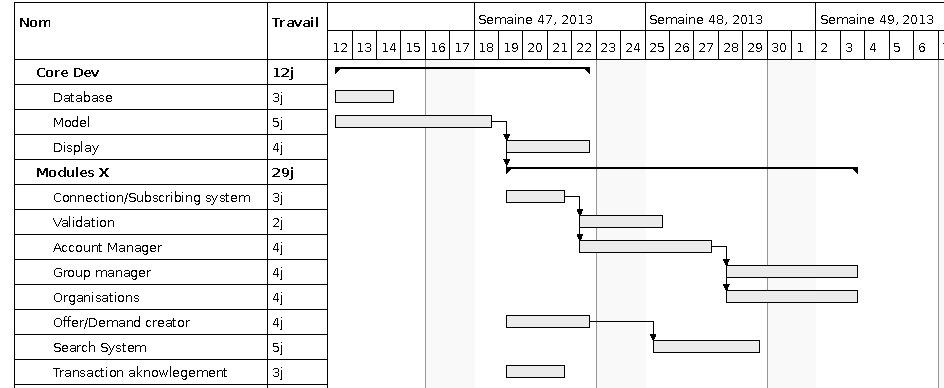
\includegraphics[width=\textwidth]{gantt_2_22_2_76.pdf}
		\caption{Gantt chart}
		\label{fig:gantt}
	\end{center}
\end{figure}

As you can see in this developpment plan diagram, we are planning on achieving the work in about a month and a half, distributed on about three weeks.
The core system should take about two weeks, then we'll be able to focus on the different modules that will use these core components to improve the user experience.
This includes smoothing everything and development of the extensions.
We tried to split each of the modules to be about the same size in terms of amount of work.
Each part should take from two to four days, the exceptions being the validation system which should take more than two days, and the core model (which is probably the biggest part and one of the most important aspect of the project) and the search system (since we decided to develop it further than a simple search system, we will try to make it very efficient and easy to use).

This kind of division allows us to have an easier approach when the time to implement will come.
Indeed, seen we all are students and not full-time IT worker, we have a lot of constraint in our agendas. 
Seen we are eight students, and thanks to the repartition of the work, once the core system will be developed, each and every one will be able to do his part of the work when he can, before the end of the project.
This diagram will help us to see what must be done earlier, so that each group can do his work when he have to (for example the search can only be done once the offer/demand creator is done).

